\clearpage
\section{Morpho-kinematics analysis}
\label{sec:morpho_kin_analysis}

\subsection{$V_{\rm{max}} /\sigma_{\rm{v}}$ distribution}

\begin{figure}[hbtp]
	\centering
	\vspace{-5pt}
	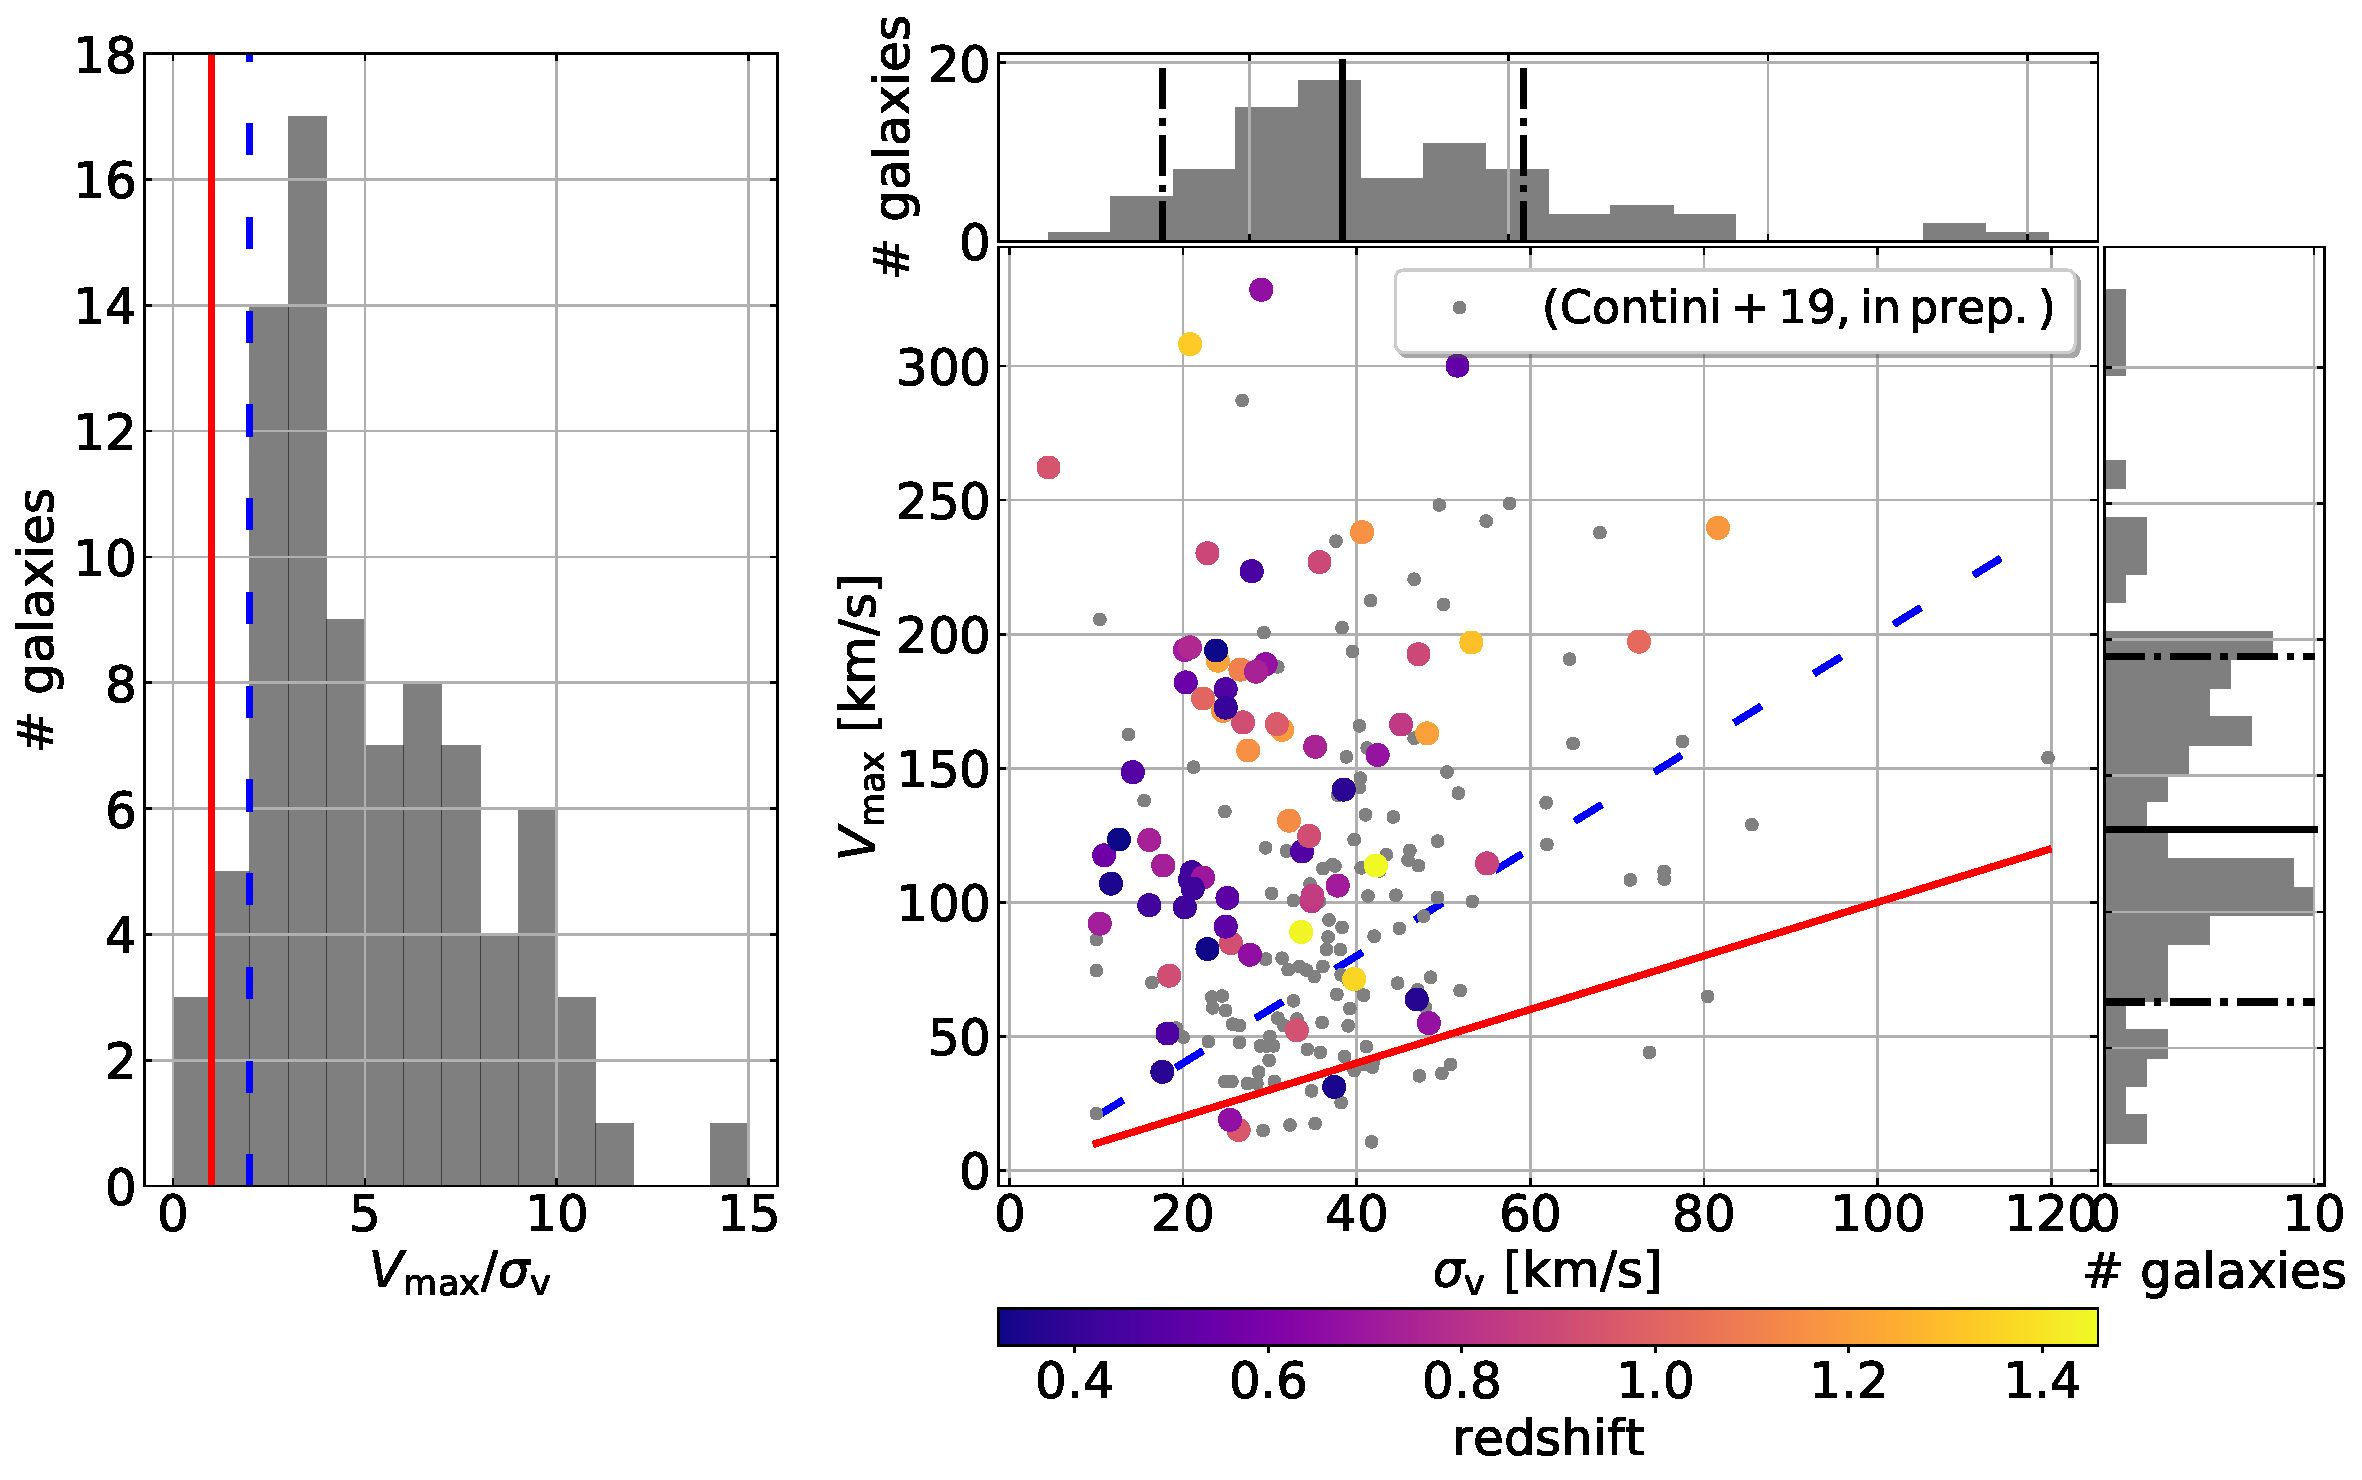
\includegraphics[width=\linewidth]{{../Plots/V_sigma}.pdf}
	\caption[$V_{\rm{max}} /\sigma_{\rm{v}}$ distribution]{Left: $V_{\rm{max}} /\sigma_{\rm{v}}$ distribution. Right: $V_{\rm{max}} - \sigma_{\rm{v}}$ diagram with galaxies colour coded according to their redshift and the corresponding distributions in terms of maximum rotation velocity and velocity dispersion (median value represented as a plain black line and the dispersion around the median as black dashed dotted lines). The sample of intermediate-redshift galaxies observed with MUSE in the HUDF (Contini et al. 2019, in preparation) is also plotted for comparison. In each plot, two lines, a red plain one for $V_{\rm{max}} /\sigma_{\rm{v}} = 1$ and a blue dashed one for $V_{\rm{max}} /\sigma_{\rm{v}} = 2$, are over-plotted to show the separation between dispersion dominated systems ($<1$) and rotationally supported galaxies ($>2$). We find that $90\%$ of our sample galaxies are rotationally supported.}
	\label{fig:Vmax_sigma}
\end{figure}

Intermediate and high redshift galaxies are classified in kinematics studies as either dispersion dominated ($V_{\rm{max}} /\sigma_{\rm{v}} < 1$) or rotationally supported ($ > 1 - 2$). The galaxies velocity dispersion is returned by the model as a parameter, as well as the turnover radius $R_{\rm{c}}$, the plateau velocity $V_{\rm{c}}$ and the largest radius where the fit was performed $R_{\rm{last}}$. To remain consistent with other studies, we decided to
\begin{enumerate*}[label=(\alph*)]
	\item compute the maximum rotation velocity of our galaxies at $R_{\rm{max}} = 2.2 R_{\rm{d}}$, with $R_{\rm{d}} \approx 0.5955 R_{1/2}$ the disc scale length (see Appendix \ref{sec:disk_scale_length} for more details).
	\item only keep galaxies with a reliable measure of $V_{\rm{max}}$, that is either if $R_{\rm{max}} < R_{\rm{last}}$ or $R_{\rm{c}} < R_{\rm{last}}$.
	
\end{enumerate*}\\

Our sample is represented in Fig.\,\ref{fig:Vmax_sigma} (coloured filled circles) and compared against the sample of intermediate-redshift galaxies observed with MUSE in the Hubble Ultra Deep Field (HUDF, Contini et al. 2019, in preparation). We find that most galaxies ($90\%$) are rotationally supported ($V_{\rm{max}} /\sigma_{\rm{v}} > 2$). This must be put in contrast with other studies where a higher fraction of dispersion dominated galaxies were found (eg. \shortciteNP{Schreiber2009}, \shortciteNP{Law2009}, \shortciteNP{Gnerucci2011}, \shortciteNP{Epinat2012}, \shortciteNP{Contini2016}). The most probable explanation for such a large fraction is that we use more restrictive selection criteria than in other works. These have removed a substantial fraction of galaxies which are spatially barely resolved with MUSE. However, less restrictive criteria, such as the size threshold in the SNR maps used in Contini et al. (2019), allow one to select small galaxies which are dominated by beam-smearing effects. Therefore, it is not that surprising to find fewer dispersion dominated galaxies in our sample.\\

We do not find any significant evolution with redshift. Visually, it seems that galaxies with higher dispersion are found at higher redshift. But splitting the sample around $\sigma_{\rm{v}} \approx 30 - \SI{40}{km/s}$ into two categories and computing the median value of the redshift for both populations does not yield a high enough redshift difference given the large dispersion.

\begin{wrapfigure}{l}{0.6\linewidth}
	\centering
	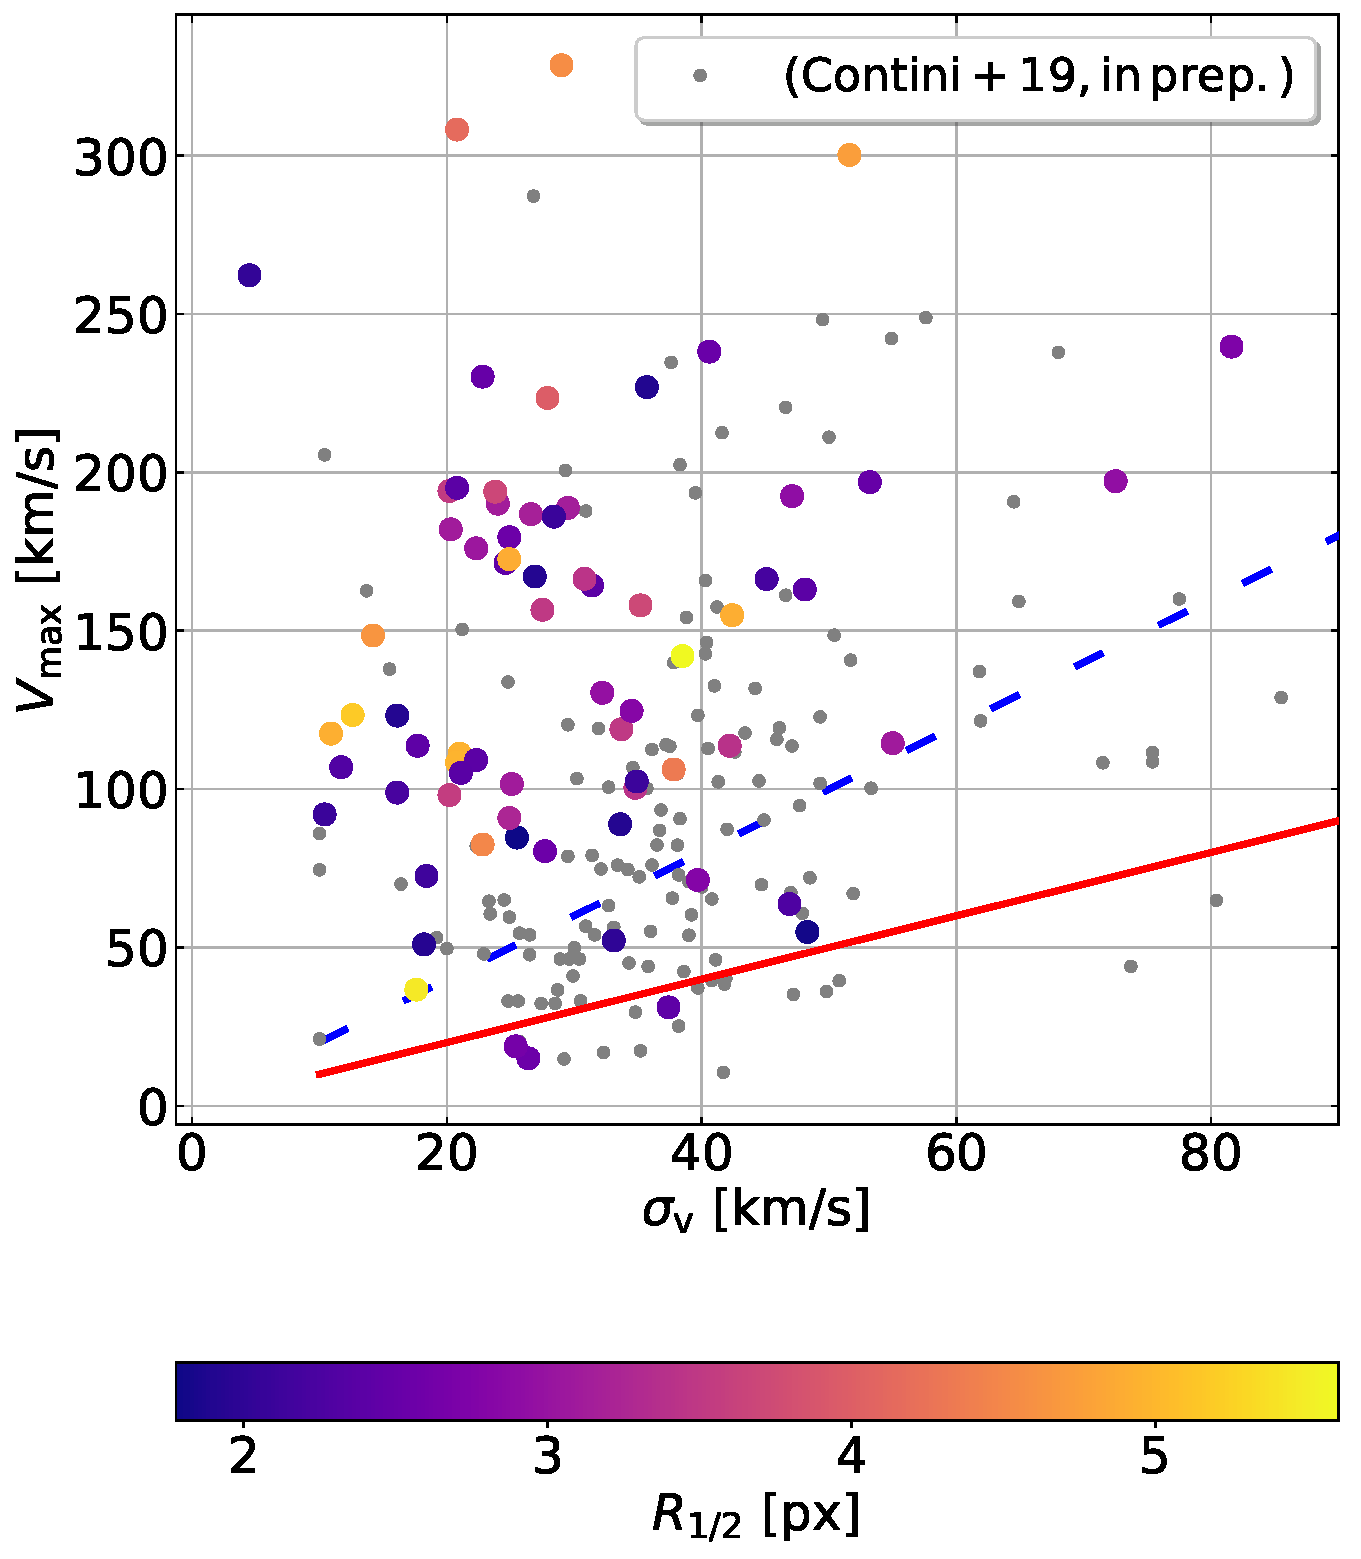
\includegraphics[width=\linewidth]{{../Plots/V_sigma_size}.pdf}
	\caption[$V_{\rm{max}} - \sigma_{\rm{v}}$ diagram as a function of apparent size]{Same graph as in Fig.\,\ref{fig:Vmax_sigma} right plot where the galaxies have been colour coded according to their apparent size on the sky. The dispersion dominated galaxies all have small sizes, but at larger radii we do not find a clear link between size and $V_{\rm{max}}$ or $\sigma_{\rm{v}}$.}
	\label{fig:V_sgima_size}
\end{wrapfigure}

We checked the effect of size selection on the $V_{\rm{max}} / \sigma_{\rm{v}}$ distribution as shown in Fig.\,\ref{fig:V_sgima_size}. We do not find a clear relation between the half-light radius and the rotation maximum velocity, nor the velocity dispersion. But, we do observe that all the dispersion dominated galaxies, as well as those classified as in between ($1 < V_{\rm{max}} / \sigma_{\rm{v}} < 2$) are all found to be among the smallest ones. Nevertheless, with less than $10$ dispersion dominated objects, it is difficult to conclude. In principle, one should perform the kinematical modelling for the unresolved, beam-smearing dominated galaxies and compare the $V_{\rm{max}} / \sigma_{\rm{v}}$ distribution of this population with ours to see how the size selection criterion would translate in terms of the proportion of dispersion dominated systems.\\

It is possible to relate the ratio between the maximum rotation velocity and the velocity dispersion to the gas fraction in galaxies. Toomre \shortcite{Toomre1964} provided an estimate of the gravitational stability of rotating gas parcels and showed that the rotation of disks ($f_{\rm{c}} \approx \Omega^2 R$) cannot counter-balance their gravity ($f_{\rm{g}} \approx \pi G \Sigma $) if their length is below $L_{\rm{crit}} = (\pi G \Sigma)/\Omega^2$. This can be compared with Jean's instability which occurs when $L > L_{\rm{J}} \approx \sigma_{\rm{v}}^2 / ( G \Sigma )$. The combination of the effects of gravitational and centrifugal accelerations are summarised in the Toomre parameter

\begin{equation}
		Q =  \frac{\kappa \sigma_{\rm{v}}}{\pi G \Sigma_{\rm{gas}}} \approx \frac{\sigma_{\rm{v}}}{f_{\rm{gas}} V_{\rm{max}}}
\end{equation}
where $\kappa \approx V_{\rm{max}} / R$ is the epicyclic frequency, $\Sigma_{\rm{gas}}$ is the gas mass surface density and $f_{\rm{gas}}$ the fraction of gas in the galaxies. In the case of marginally stable disks ($Q \approx 1$) there should therefore be a correlation between $V_{\rm{max}}$ and $\sigma_{\rm{v}}$, though with some scatter as disks will have slightly different gas fractions (see \shortciteA{Tacconi2018}; \shortciteA{Freundlich2019}).




%\newpage
\subsection{Tully-Fisher Relation}

\subsubsection{Recovering the TFR}

\begin{figure}[htbp]
	\centering
	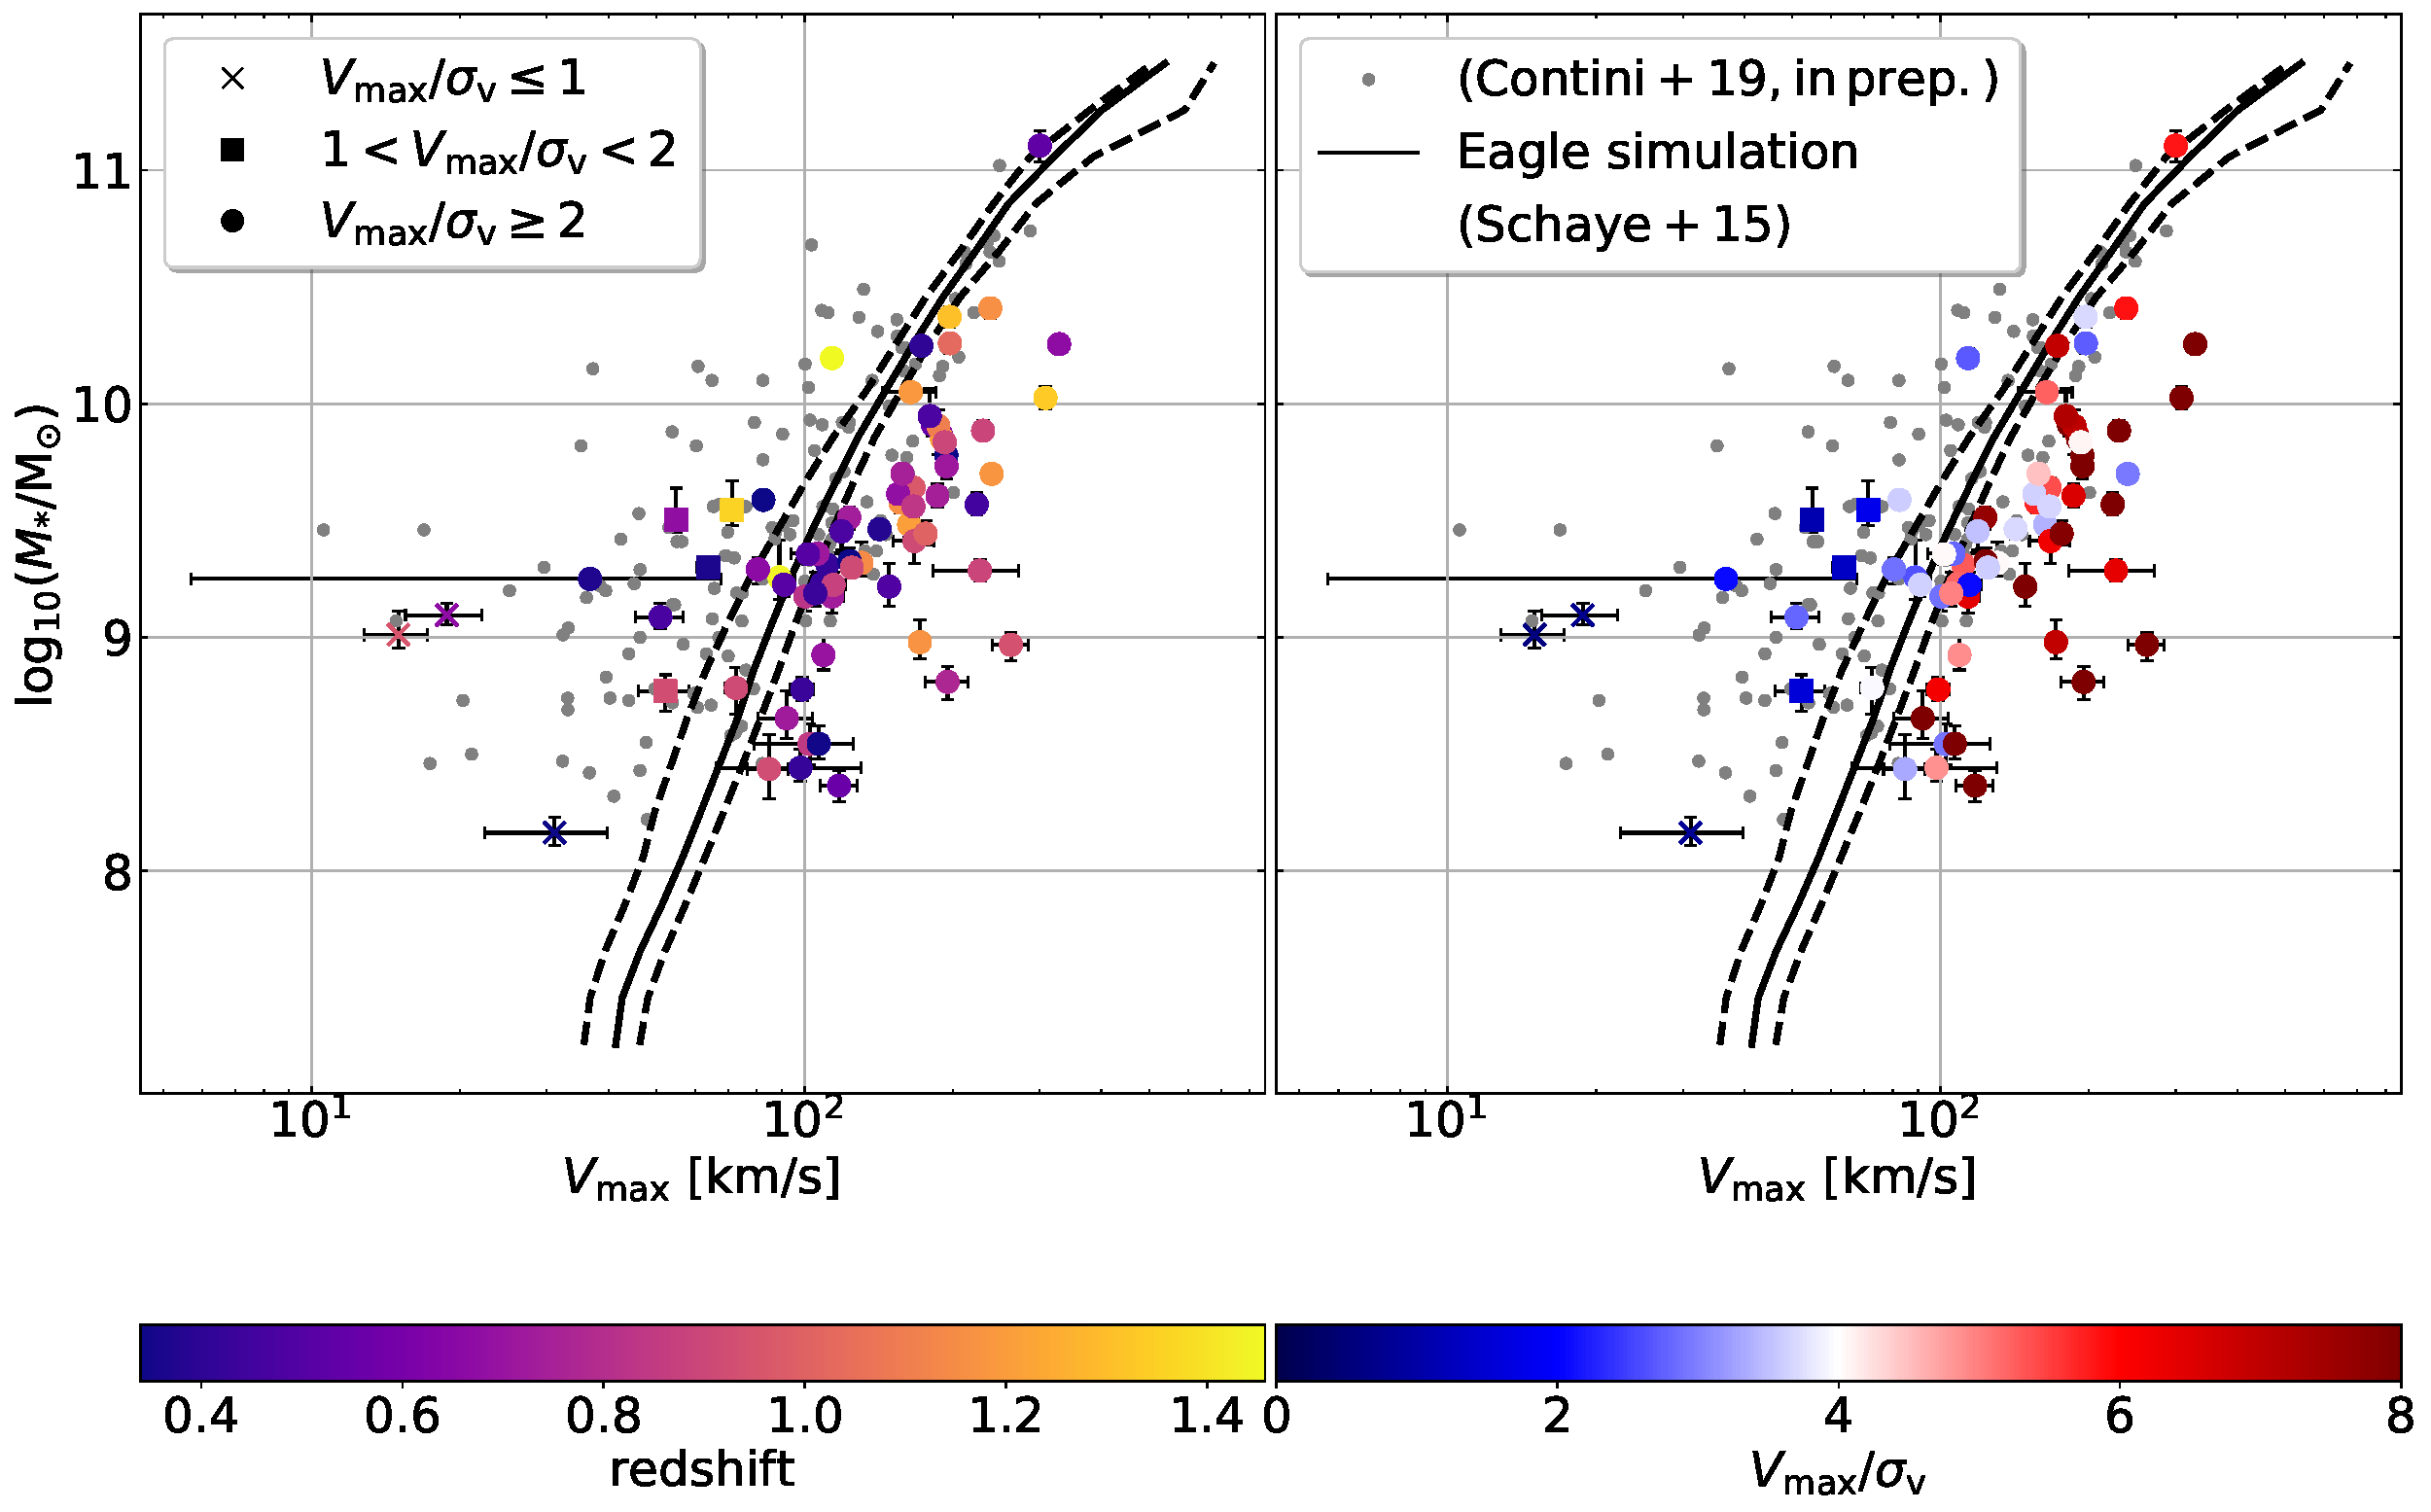
\includegraphics[width=\linewidth]{{../Plots/TFRz}.pdf}
	\caption[Tully-Fisher Relation]{Tully-Fisher Relation
	\begin{enumerate*}[label=]
		\item Left: as a function of redshift.
		\item Right : as a function of $V_{\rm{max}} /\sigma_{\rm{v}}$ ratio.
	\end{enumerate*}		
	In both plots, galaxies have been separated between rotationnaly supported (filled circle), dispersion dominated (cross) and in between (filled square). Error bars correspond to $1\sigma$ uncertainties. The TFR from the EAGLE simulation \shortcite{Schaye2015} and its errors (plain and dashed lines) are over-plotted for comparison. We also over-plotted (grey points) the results of Contini et al., 2019 (in preparation) for galaxies at similar redshifts observed with MUSE in the HUDF.}
	\label{fig:TFR}
\end{figure}

We recover the Tully-Fisher Relation (TFR) of our sample galaxies by comparing their stellar masses, obtained with SED fitting and given in \shortciteA{laigle_cosmos2015_2016} catalogue, against the maximum (inclination corrected) rotation velocity. In Fig.\,\ref{fig:TFR}, we compare our TFR with the one derived from the EAGLE suite of hydrodynamical simulations \shortcite{Schaye2015} of galaxies in a similar mass range. We also add the results obtained in Contini et al. (2019) discussed in the previous section.\\

We find a similar trend between mass and rotation velocity, but globally with an offset towards larger velocities with respect to both the simulations and the MUSE observations in the HUDF. This is consistent with the $V_{\rm{max}} / \sigma_{\rm{v}}$ distribution, but also with the lack of dispersion dominated galaxies. Such objects are at the origin of the dispersion in the TFR at lower rotation velocities and lower masses in Contini et al. (2019) sample in Fig.\,\ref{fig:TFR}. We can also see this effect in our sample where the galaxies with the lowest $V_{\rm{max}} / \sigma_{\rm{v}}$ ratio are the most scattered towards lower rotation velocities (see right plot of Fig\,\ref{fig:TFR}). In terms of redshift, we do not find any evolution of the TFR zeropoint. 


\subsubsection{A size dependent relation ?}

\begin{wrapfigure}{r}{0.6\linewidth}
	\centering
	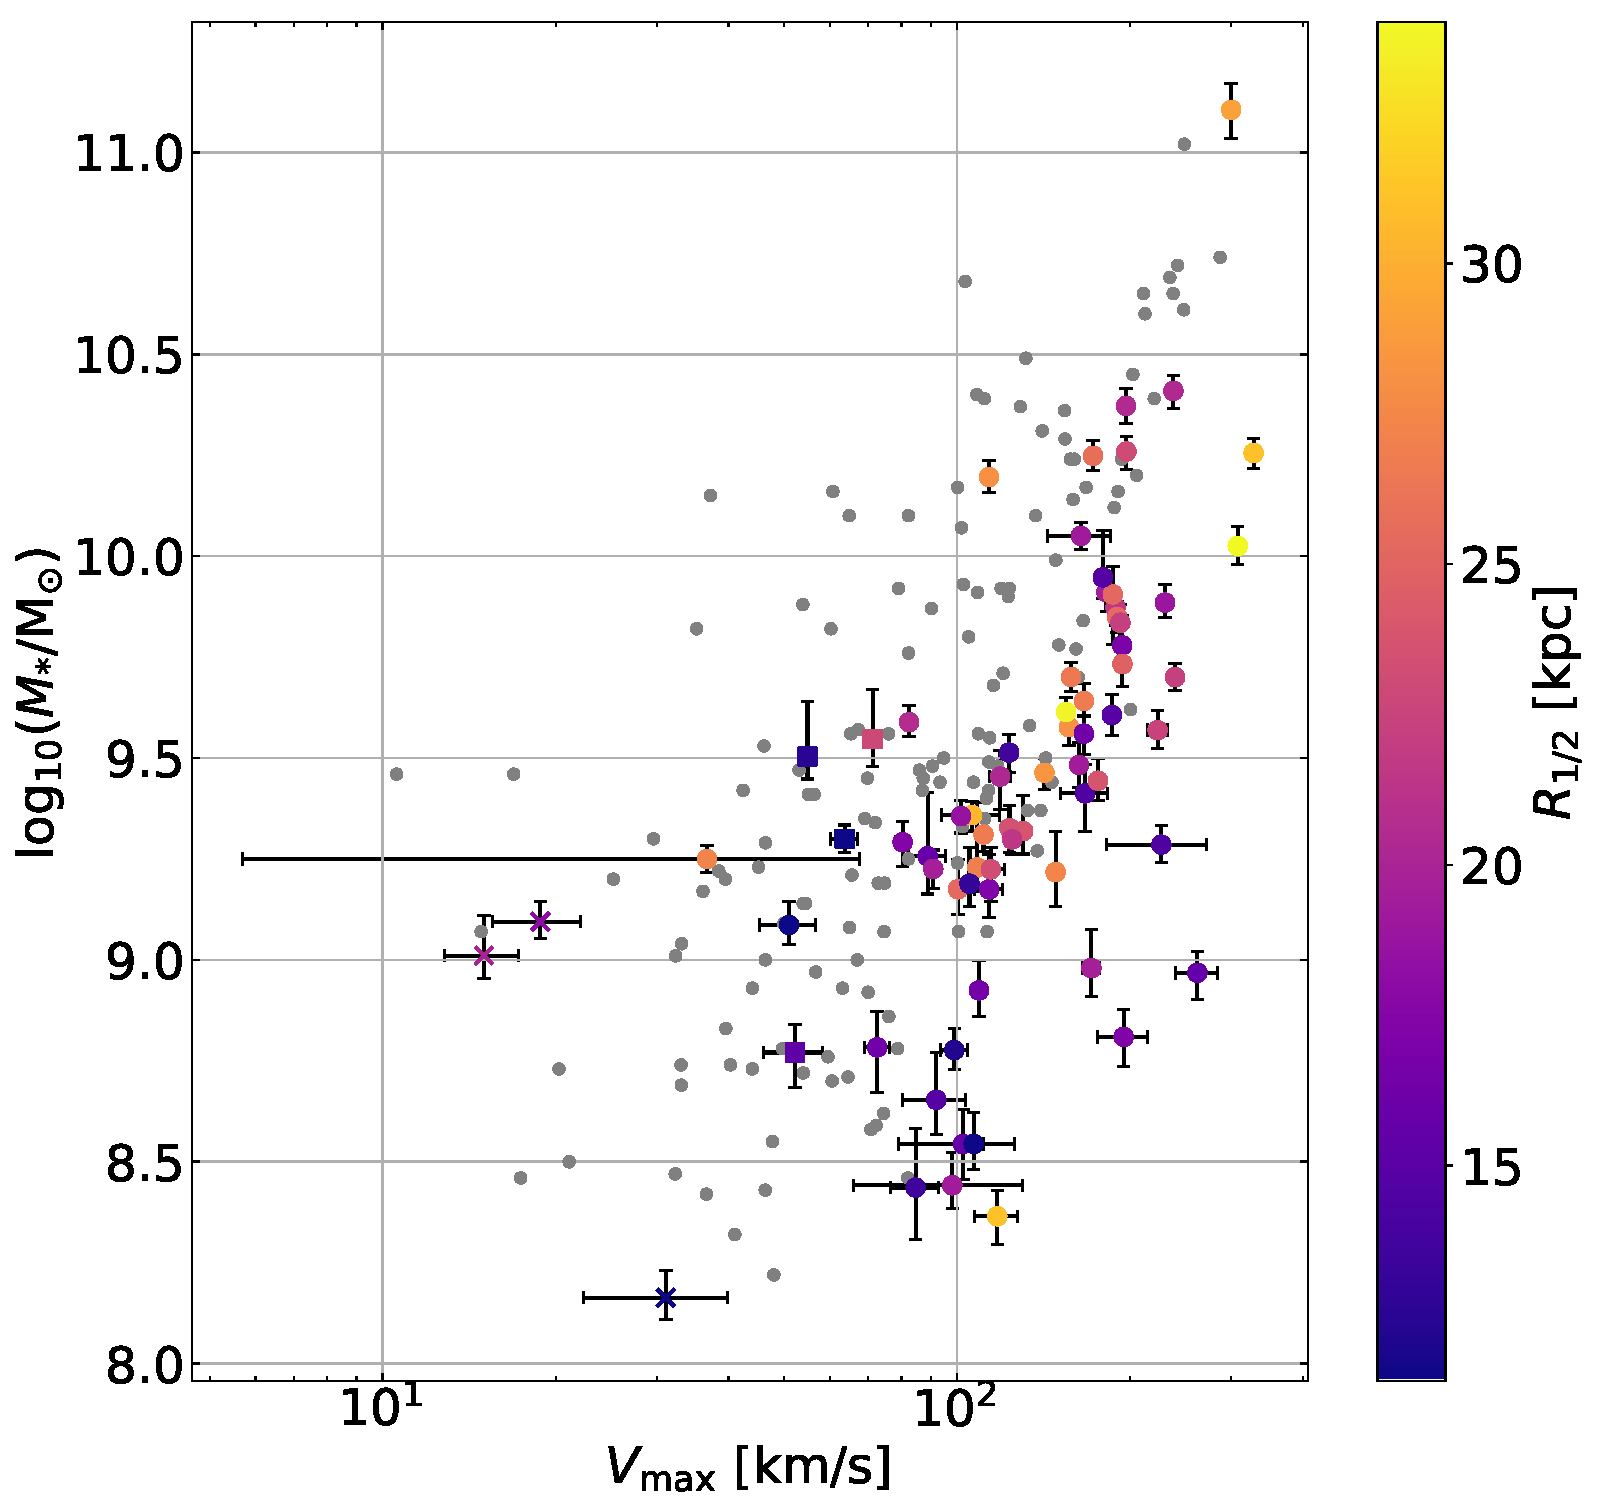
\includegraphics[width=\linewidth]{{../Plots/TFR_sizeKPC}.pdf}
	\caption[TFR as a function of galaxies physical size]{Same plot as Fig\,\ref{fig:TFR} (similar legend) but galaxies are colour coded according to their physical size as computed from Eq.\,\ref{eq:TFR_phys_size}. We observe a tendency for larger galaxies to be located further up on the TFR (larger masses and rotation maximum velocity).}
\end{wrapfigure}

There does not seem to be any obvious correlation between the TFR of our sample and the galaxies redshift or the angular size as can be seen in Fig.\,\ref{fig:TFR_sizePX}. However, we do expect to see a correlation between their stellar mass and their size \shortcite{Mowla2018}. Thus, knowing their angular half-light radius (we will note it $\theta_{1/2}$) and their redshift, we derived their physical size (half-light radius in $\si{kpc}$, we note it $R_{1/2}$ from now on)

\begin{equation}
	R_{1/2}(z) = \theta_{1/2} d_A (z)
	\label{eq:TFR_phys_size}
\end{equation}

with $d_A (z) = d_c(z) / (1+z)$ the angular diameter distance and $d_c$ the comoving distance. As expected, smaller galaxies have a lower mass and, given the TFR, also have a lower maximum rotation velocity.

\subsubsection{The effect of inclination}

Our TFR in Fig\,\ref{fig:TFR} contains the whole sample of spatially resolved galaxies. Even though the maximum rotation velocity is corrected of the inclination through Eq.\,\ref{eq:V_obs_max}, it still has an impact on the TFR. The kinematics of edge-on galaxies (typically $i \gtrsim 70\degree$) is less constrained because
\begin{enumerate*}[label=(\alph*)]
	\item of the lack of pixels to fit the model.
	\item the assumption of an infinitely thin disc on which is based the model is not necessarily met any more.
\end{enumerate*}
For face-on galaxies ($i \lesssim 30\degree$), we do generally have plenty of pixels (assuming it is spatially extended enough), but the measured velocity on the line of sight is also smaller, which requires a better spectral resolution to produce detailed velocity field maps. In addition to that, the relative error on the inclination is greater when it approaches $0\degree$ as morphological models can easily converge towards non-zero values of $b/a$ (see left plot of Fig.\,\ref{fig:erreur_inclinaison}). We therefore checked how the inclination might have impacted our previous TFR. In Fig.\,\ref{fig:TFR_inc} we separated our galaxies into two categories: face-on and edge-on galaxies with less constrained kinematics, and those with reasonable values of inclination ($30\degree \leq i \leq 70\degree$). Only rotationnaly supported galaxies with $V_{\rm{max}} / \sigma_{\rm{v}}$ are eliminated with this criterion. This is not very surprising since edge-on galaxies need to have a clear disk-like structure to be classified as such, which is generally linked to larger values of rotation velocity. In addition, we expect to have a significant fraction of galaxies with a maximum rotation velocity above the TFR because of the effect of very low inclinations on the sky.


\subsection{Scaling between $\rm{SFR}$ and velocity dispersion}

\begin{wrapfigure}{l}{0.6\linewidth}
	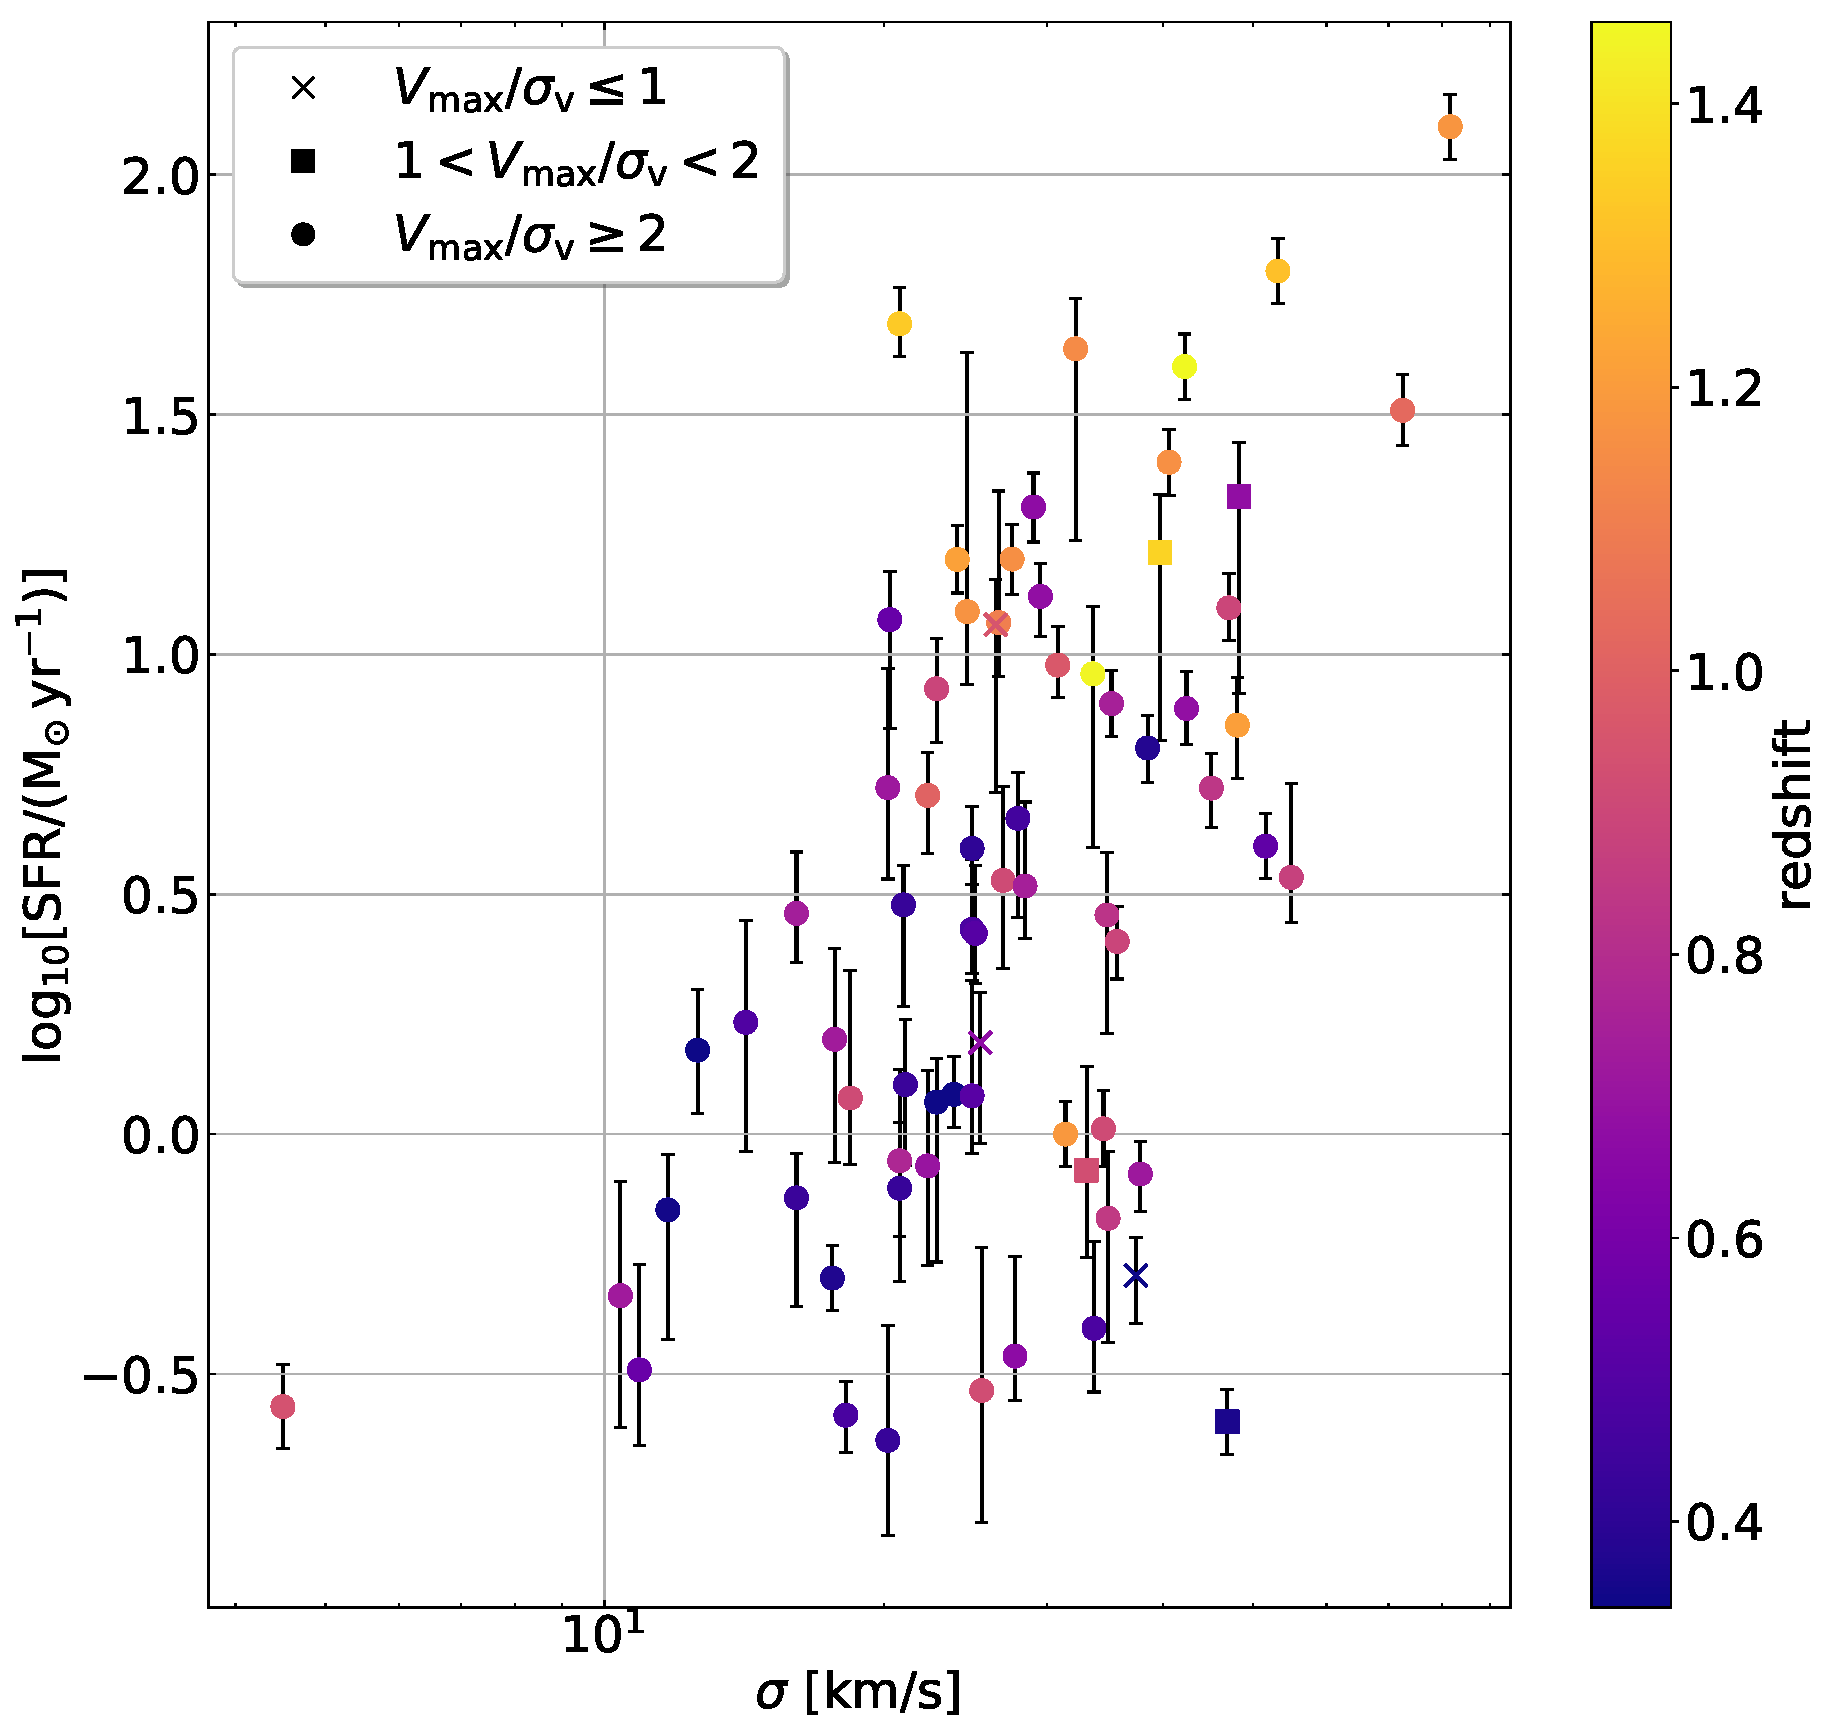
\includegraphics[width=\linewidth]{{../Plots/SFR_sigma}.pdf}
	\caption[Scaling between SFR and $\sigma_{\rm{v}}$]{Scaling relation between the star formation rate and the velocity dispersion. We find an evolution as in the $\rm{SFR} - V_{\rm{max}}$ diagram, but with more scatter}
	\label{fig:SFR_sigma}
\end{wrapfigure}

Since our galaxies are all located on the main sequence, there exists a relation between the $\rm{SFR}$ and the mass, with more massive galaxies having higher star formation rates. Given the TFR, we also have a scaling between mass and maximum rotation velocity. Therefore, it seems natural to see a link between the $\rm{SFR}$ and the rotation velocity in Fig.\,\ref{fig:SFR_Vmax}. Interestingly enough, we do observe a redshift evolution. This is mainly due to the redshift evolution of the $\rm{SFR}$ on the main sequence (see Fig.\,\ref{fig:sfr_vs_mass}). If we observe such a relation, one may ask if higher a $\rm{SFR}$ leads to higher velocity dispersion as well. In Fig.\,\ref{fig:SFR_sigma}, we show the variation of the $\rm{SFR}$ with the velocity dispersion and with redshift. Qualitatively, we can see that the velocity dispersion seems to increase with $\rm{SFR}$ and with redshift, as discussed before, though the scatter is higher than between the $\rm{SFR}$ and $V_{\rm{max}}$. A similar trend, both in terms of $\rm{SFR} - \sigma_{\rm{v}}$ relation and redshift evolution on this sequence, was recently found by \shortciteA{Hung2019} in cosmological simulations from the FIRE project \shortcite{Hopkins2014}. Moreover, if we interpret the velocity dispersion as the effect of energy injection into the gas, it seems consistent to find larger values for higher $\rm{SFR}$. This is the conclusion reached by \shortciteA{Lehnert2013} who compared data obtained with SINFONI with simulations of gas rich galaxies, and who found that most of the velocity dispersion was driven by star formation.
